\chapter{Constructive Heuristics}

\section{Greedy}\label{sec:greedy}
Greedy heuristic for TSP start by choosing a random element and add one node at a time the closer node, making as usual the local optimal choice. This create good path in the first part of the tour, however the last added edges create different crosses with the other one. Therefore this heuristic can be applied in combination with refining heuristics such as: local branch, hard fixing, iterative two opt and other ones that try to improve a tour.\\
The algorithm is $ O(n^2) $ where $ n = |V| $, therefore is pretty fast, however depending on the first selected node, the cost of the tour can differ more than 100 \% one another. The implemented algorithm, at cost of execution time, perform the described greedy using all the nodes as starting node, returning the shortest tour. The time complexity for the implemented algorithm raise to $ O(n^3) $.\\
In fig \ref{fig:a280_10_} an example of tour calculated with the implemented algorithm.

\begin{figure}[h]
	\centering
	\centering
	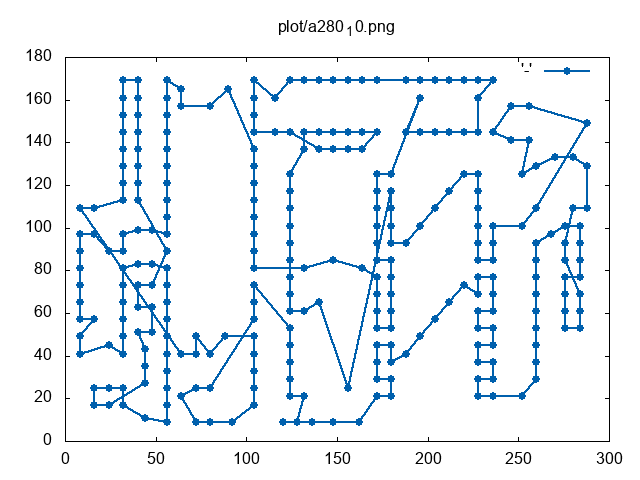
\includegraphics[width=0.7\columnwidth]{../res/a280_10.png}
	\caption{The shortest greedy tours.}
	\label{fig:a280_10_}
\end{figure}



\subsection{Greedy with CGAL Library}
To take a look at the potential of the CGAL library, we decided to implement the greedy algorithm. It follows the same idea as the one previously described (Section \ ref {sec: greedy}) but using completely different data structures. Thanks to the potential of the C ++ code and therefore the use of objects, the CGAL library offers a very wide range of elements.\\ First of all, the objects used for this algorithm are briefly explained:
\begin{enumerate}
\item CGAL :: Simple\_cartesian <double> K: 
\item CGAL :: Search\_traits\_2 <K> TreeTraits:
\item CGAL :: Orthogonal\_k\_nemap.com\_search <TreeTraits> Neighbor\_search:
\item Neighbor\_search :: Tree Tree:
\end{enumerate}

\section{Greedy Randomize Adaptive Search Path (GRASP)}
GRASP metaheuristic, as the name anticipate, is a Greedy constructive heuristic with some randomization. Indeed, for the TSP problem, instead of bring the closer isolated node as next, it's chose a random node between the $ G $ closest isolated nodes, where $ G = 3 $ in the tested implementation.
The idea is that in TSP it's not always the closer to be the next node on the optimum tour. Moreover, in other metaheuristics that start from a solution and optimize it, a percentage of randomness is appreciated.

In figure \ref{fig:att48_diff} can be compared of the optimum tour, the best Greedy and 4 different instances of GRASP. It's nice to see that the best Greedy (fig \ref{fig:att48_GREEDY}) is pretty close to the optimal solution and also some instance of GRASP like \ref{fig:att48_GRASP2} and \ref{fig:att48_GRASP4}.
\begin{figure}[!h]
	\begin{subfigure}{.5\textwidth}
		\centering
		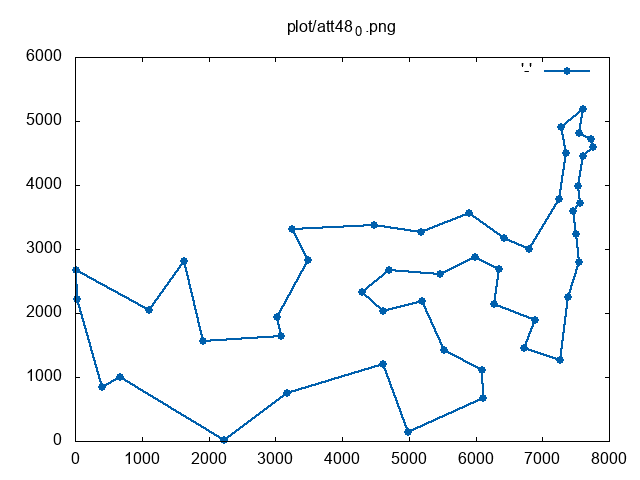
\includegraphics[width=\columnwidth]{../res/att48_0.png}
		\caption{Optimal subtour (cost $ = 10628 $, exec time = $ 0.76 $ s)}
		\label{fig:att48_best}
	\end{subfigure}
	\begin{subfigure}{.5\textwidth}
		\centering
		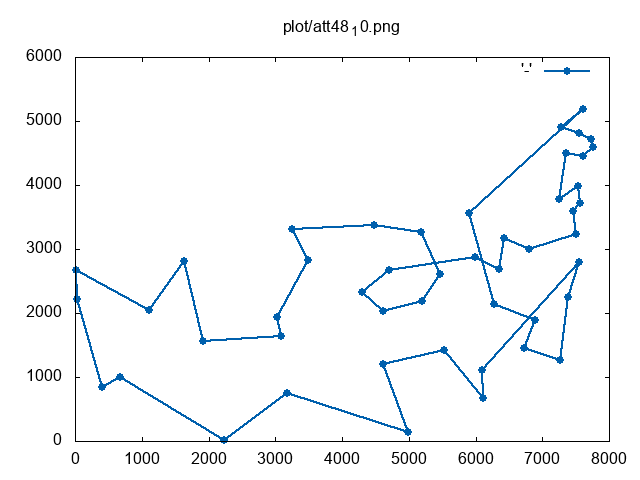
\includegraphics[width=\columnwidth]{../res/att48_10.png}
		\caption{Best Greedy (cost $ = 12012 $, exec time = $ 10^{-6} $s)}
		\label{fig:att48_GREEDY}
	\end{subfigure}
	\begin{subfigure}{.5\textwidth}
	\centering
	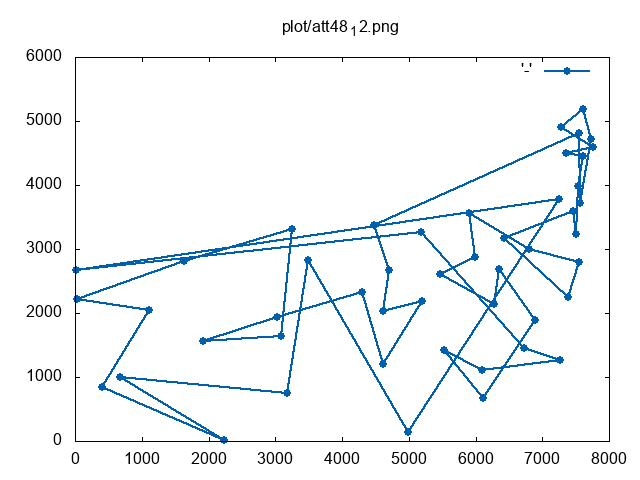
\includegraphics[width=\columnwidth]{../res/att48_12_1.png}
	\caption{GRASP (cost = 21824, exec time = $ 10^{-6} $s)}
	\label{fig:att48_GRASP1}
	\end{subfigure}
	\begin{subfigure}{.5\textwidth}
	\centering
	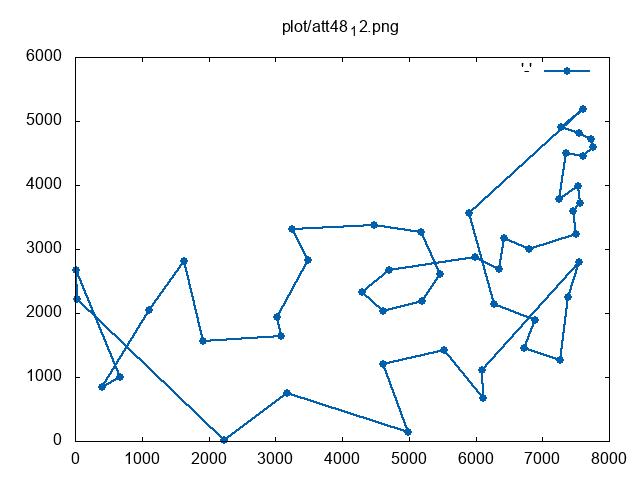
\includegraphics[width=\columnwidth]{../res/att48_12_2.png}
	\caption{GRASP (cost = 12576, exec time = $ 10^{-6} $s)}
	\label{fig:att48_GRASP2}
	\end{subfigure}
	\begin{subfigure}{.5\textwidth}
	\centering
	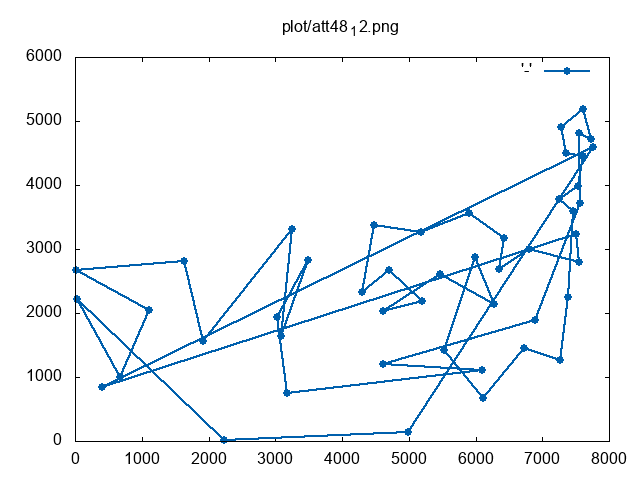
\includegraphics[width=\columnwidth]{../res/att48_12_3.png}
	\caption{GRASP (cost = 22179, exec time = $ 10^{-6} $s)}
	\label{fig:att48_GRASP3}
	\end{subfigure}
	\begin{subfigure}{.5\textwidth}
	\centering
	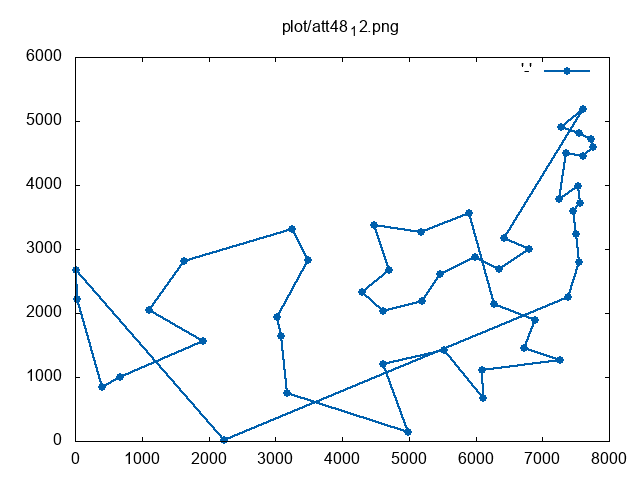
\includegraphics[width=\columnwidth]{../res/att48_12_4.png}
	\caption{GRASP (cost = 13198, exec time = $ 10^{-6} $s)}
	\label{fig:att48_GRASP4}
	\end{subfigure}
	\caption{Differences of Greedy and GRASP tour for att48.tsp instace.}
	\label{fig:att48_diff}
\end{figure}


\section{Insertion Heuristic}
Te idea of this constructive heuristic is to create an initial simple tour of 3 nodes randomly and insert one node at a time, breaking the edge that minimize the final tour cost.\\
The complexity of the algorithm is $ O(n^2) $.


\textbf{Construction heuristic comparison.} The performance profile in fig \ref{fig:pp_Lconstructives} show the three constructive presented in this chapter and plus \texttt{greedy\_best\_two\_opt} and \texttt{insertion\_best\_two\_opt}. These last two algorithm combine the constructive heuristic with the iteration of \texttt{2\_opt()} to quickly improve the cost of the solution. Between the three constructive \texttt{heristic\_insertion} is clearly better in term of time domain and optimum tour, however with the help of 
\texttt{best\_two\_opt}, \texttt{greedy} perform better than the \texttt{insertion}.\\
Another consideration is about execution time of \texttt{heuristic\_insertion} which perform better as grasp (as expected) but in term of solution cost reaches the improved version \texttt{insertion\_best\_two\_opt}

\begin{figure}[!h]
	\centering
	\begin{subfigure}{.9\textwidth}
		\centering
		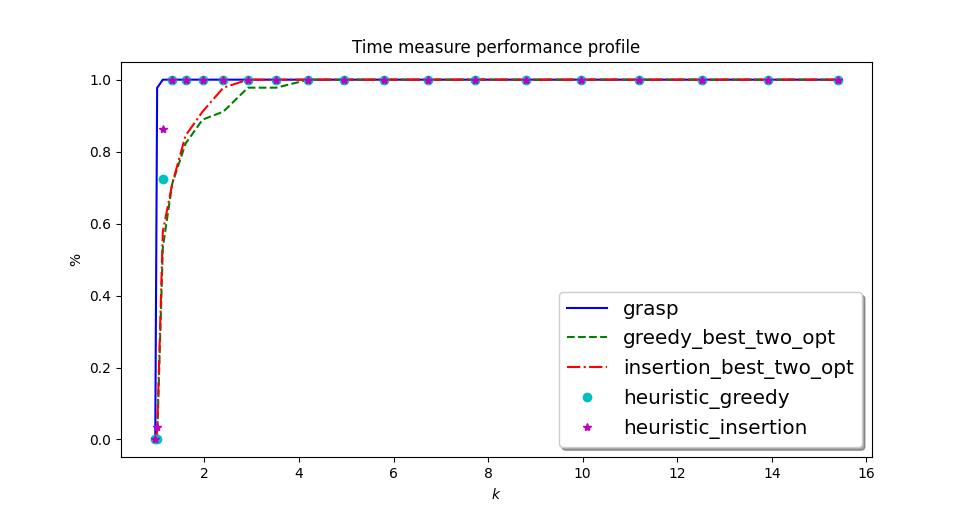
\includegraphics[width=\columnwidth]{../res/Lconstructives_time.png}
		\caption{Performance profile in time domain.}
		\label{fig:Lconstructives_time}
	\end{subfigure}
	\begin{subfigure}{.9\textwidth}
	\centering
	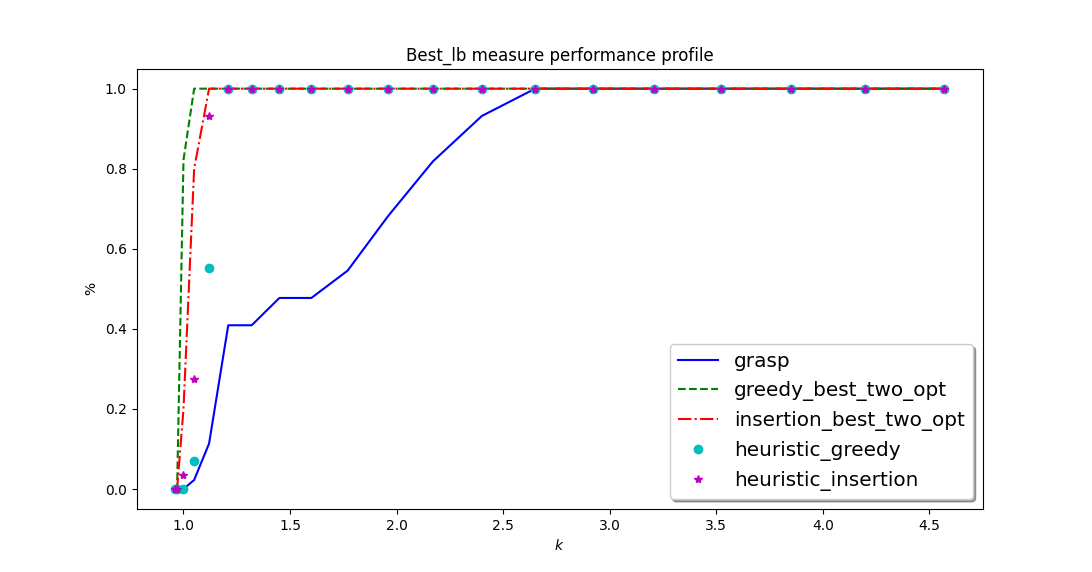
\includegraphics[width=\columnwidth]{../res/Lconstructives_lb.png}
	\caption{Performance profile in solution cost domain.}
	\label{fig:Lconstructives_lb}
	\end{subfigure}
	\caption{Performance profile of constructive heuristic}
	\label{fig:pp_Lconstructives}
\end{figure}
